\begin{frame}{Quadraturregeln: Flächen näherungsweise berechnen}
    Gesucht ist die Fläche unter einem Funktionsgraphen zwischen $a$ und $b$.
    Der Graph liegt dabei auf oder oberhalb der $x$-Achse.
    \begin{itemize}
        \item Wir teilen den Bereich in $n$ gleich breite Teilintervalle.
        \item Jedes Teilintervall hat die Breite $h=(b-a)/n$.
        \item Wir ersetzen die Fläche durch Rechtecke oder Trapeze und addieren deren Flächeninhalte.
    \end{itemize}
\end{frame}

\begin{frame}[fragile]{Vorgestelltes Beispiel: linke Riemannsumme}
    Die Höhe jedes Rechtecks ist der Funktionswert am linken Endpunkt.
    \begin{lstlisting}[language=Python, basicstyle=\ttfamily\small]
def linke_riemannsumme(f, a, b, n):
    summe = 0
    breite = (b - a) / n

    for i in range(n):
        x = a + i * breite
        hoehe = f(x)
        summe += breite * hoehe

    return summe
    \end{lstlisting}
\end{frame}

\begin{frame}{Neue Idee: Mittelpunktsregel}
    \begin{itemize}
        \item Die Breite der Rechtecke bleibt gleich.
        \item Für die Höhe verwenden wir den Funktionswert in der Mitte des Teilintervalls.
        \item Der Mittelpunkt liegt eine halbe Rechteckbreite rechts vom linken Endpunkt.
    \end{itemize}
\end{frame}

\begin{frame}{Auftrag}{Mittelpunktsregel selbst implementieren}
    \aufgabebox{1.1}
    \begin{itemize}
        \item Ergänzen Sie das Codegerüst im Skript.
        \item Vergleichen Sie für $f(x)=x^2$ auf $[0,1]$ mit $n=4$ die Mittelpunktsregel mit der linken Riemannsumme.
        \item Prüfen Sie auch $g(x)=x+1$ auf $[1,3]$.
    \end{itemize}
\end{frame}

\begin{frame}{Neue Idee: Trapezregel}
    \begin{itemize}
        \item Wir verbinden die Funktionswerte an den beiden Endpunkten durch eine gerade Strecke.
        \item Darunter entsteht ein Trapez.
        \item Sein Flächeninhalt ist die Breite multipliziert mit dem Mittelwert der beiden Höhen.
    \end{itemize}
    \[
        A_{\text{Trapez}} = h\cdot\frac{f(\text{links})+f(\text{rechts})}{2}
    \]
\end{frame}

\begin{frame}{Auftrag}{Trapezregel selbst implementieren}
    \aufgabebox{1.2}
    \begin{itemize}
        \item Ergänzen Sie das Codegerüst im Skript.
        \item Vergleichen Sie für $f(x)=x^2$ auf $[0,1]$ mit $n=4$ die Trapezregel mit der Mittelpunktsregel.
        \item Prüfen Sie auch $g(x)=x+1$ auf $[1,3]$ und begründen Sie das Ergebnis.
    \end{itemize}
\end{frame}

\begin{frame}{Monte Carlo: Zufällige Höhen mitteln}
    \textbf{Flächeninhalt = Intervallbreite mal mittlere Höhe}
    \begin{itemize}
        \item Wählen Sie $n$ Stellen $X_i$ unabhängig und gleichverteilt aus $[a,b]$.
        \item Berechnen Sie die Höhen $f(X_i)$ und deren Mittelwert.
        \item Multiplizieren Sie die mittlere Höhe mit der Breite $b-a$.
    \end{itemize}
    \[
        A\approx (b-a)\cdot\frac{1}{n}\sum_{i=1}^{n}f(X_i)
    \]
    Auf $[0,1]$ genügt der Mittelwert. Zufällige $y$-Koordinaten sind nicht nötig.
\end{frame}

\begin{frame}{Monte Carlo: Treffer zählen}
    \begin{itemize}
        \item Erzeugen Sie $n$ gleichverteilte Zufallspunkte im Einheitsquadrat.
        \item Zählen Sie, wie viele Punkte in der gesuchten Fläche liegen.
        \item Treffer zählen als $1$, alle anderen Punkte als $0$. Ihr Mittelwert ist der Trefferanteil und schätzt die Fläche im Einheitsquadrat.
    \end{itemize}
    \[
        A\approx\frac{\text{Anzahl Treffer}}{n}\cdot 1
    \]
    Mehr Punkte verringern typische Zufallsschwankungen, garantieren aber nicht in jedem Durchlauf ein genaueres Ergebnis.
\end{frame}

\begin{frame}{Fläche zwischen zwei sich kreuzenden Graphen}
    \[
        f(x)=0.5+0.4\sin(4\pi x),\qquad
        g(x)=0.5+0.4\cos(4\pi x)
    \]
    \begin{center}
        % TikZ verwendet Grad; 4*pi*x im Bogenmass entspricht 720*x Grad.
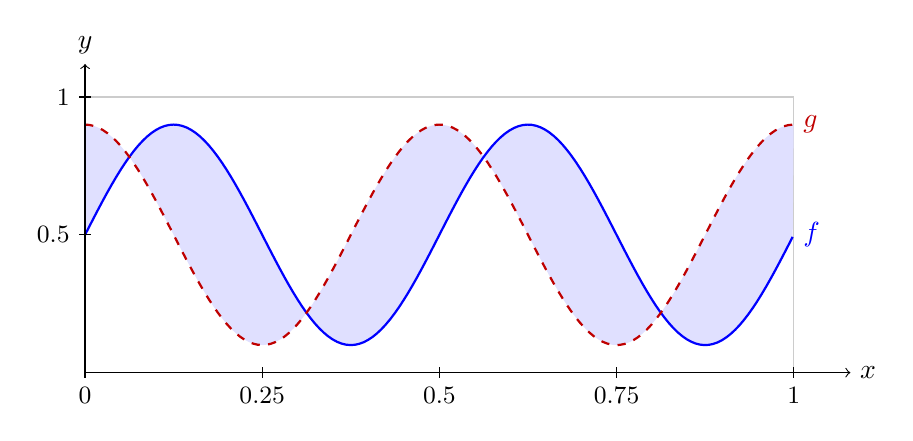
\begin{tikzpicture}[x=9cm, y=3.5cm]
    \draw[gray!40] (0,0) rectangle (1,1);
    \path[fill=blue!12]
        plot[domain=0:1, samples=161] (\x,{0.5+0.4*sin(720*\x)})
        -- plot[domain=1:0, samples=161] (\x,{0.5+0.4*cos(720*\x)})
        -- cycle;
    \draw[blue, thick] plot[domain=0:1, samples=161]
        (\x,{0.5+0.4*sin(720*\x)});
    \draw[red!75!black, thick, dashed] plot[domain=0:1, samples=161]
        (\x,{0.5+0.4*cos(720*\x)});
    \draw[->] (0,0) -- (1.08,0) node[right] {$x$};
    \draw[->] (0,0) -- (0,1.12) node[above] {$y$};
    \foreach \x in {0,0.25,0.5,0.75,1}
        \draw (\x,0.02) -- (\x,-0.02) node[below] {\small $\x$};
    \foreach \y in {0.5,1}
        \draw (0.008,\y) -- (-0.008,\y) node[left] {\small $\y$};
    \node[blue, right] at (1,0.5) {$f$};
    \node[red!75!black, right] at (1,0.9) {$g$};
\end{tikzpicture}

    \end{center}
    Gesucht ist die Summe aller schattierten Teilflächen auf $[0,1]$.
\end{frame}

\begin{frame}{Auftrag}{Fläche zwischen zwei Graphen}
    \aufgabebox{1.3}
    \begin{itemize}
        \item Monte Carlo: Zählen Sie Punkte zwischen den Graphen. Alternativ mitteln Sie die Abstände $|f(X_i)-g(X_i)|$ an zufälligen Stellen.
        \item Trapezregel: Verwenden Sie den senkrechten Abstand der Graphen als Höhe.
        \item Vergleichen Sie die Näherungen mit $A\approx 0.3601265265$.
        \item Warum genügt es nicht, die beiden Flächen unter den Graphen voneinander abzuziehen?
    \end{itemize}
\end{frame}
